\chapter{Related work}
In this chapter we survey the studies which focus on problem of irradiance estimation using sky images. The usage of ground-based cameras for studying effect of clouds on irradiation has a long history, as early as 1977 when Borkowski et al.\cite{Borkowski1977} developed the first whole-sky camera system for investigating effects of clouds on middle ultraviolet global radiation. In this study, the degree of solar obstruction and cloud coverage were determined visually from the images. Later in 1998, Jeff Sabburg and Joe wong\cite{Sabburg1998} developed and evalued the first automated, ground-based, sun-centered sky camera system for cloud assessment. However, since the purpose of study was the clouds effect on UVB\footnote{Ultraviolet B} radiation they only considered a small area around the sun for cloud and sun ostruction detection which is of paramount importance for this rays. They use a threshold-based approch on gray scale pixel intensities for cloud detection. They also use solar radiation measurements in a image processing algorithm to reduce reflections from the sun on the camera system being mistaken for cloud in the images.

\section{Estimate irradiance from zone types in sky images}
One of the recent researches done in this area is held as a collaboration between Universitatea Transilvania din Braşov in Romania and Cyprus University of Technology\cite{romania_paper}\cite{romania_report}.This work uses sets of two sensequative images taken by wdie-view angle GoPro Hero2 camera(one with normal exposure and the other one under-exposed) and extracts their RGB\footnote{(Red, Green, Blue)}, HSV\footnote{(Hue, Saturation, Value)} components. Then by learning several intensity ranges, they segment four zone type in each image: sun, blue sky, thin clouds and thick clouds. One sample of segmentaion is shown in figure\ref{fig:capatitati}.

\begin{figure}[h]
\caption{Three different zones identified in images (sun, cloud, sky)}
\label{fig:capatitati}
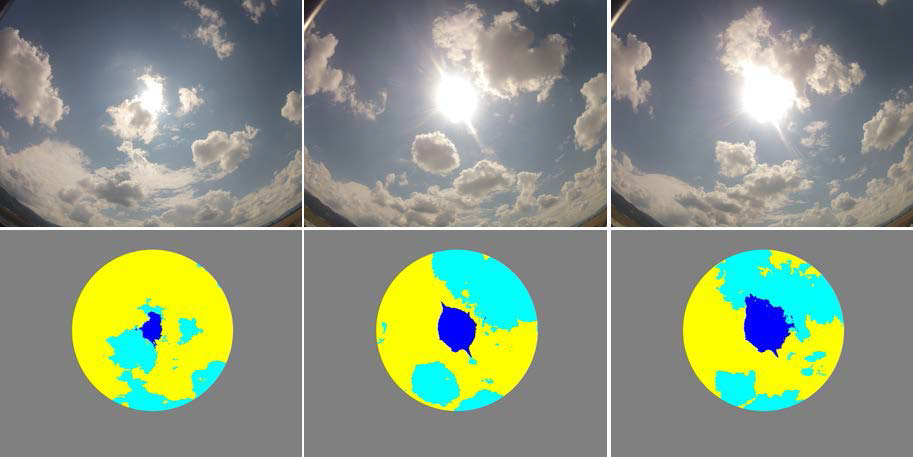
\includegraphics[scale=.5]{capatitati}
\centering
\end{figure} 

 The irradiance (direct, diffuse, global) is recorded using the equipment Kipp \& Zonen, Solys2 at the same time of image capturing. Finally, a regressor used to estimate direct irradiation (DNI) based on a feature vector consisting the number of pixels of different zone types in the images. The correlation in the result is shown in figure\ref{fig:w1_predict}.

\begin{figure}[h]
\caption{Correlation between estimated DNI and recorded DNI.}
\label{fig:w1_predict}
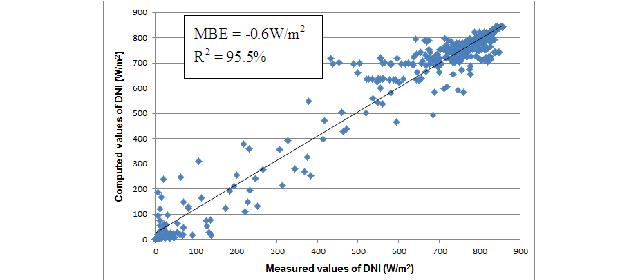
\includegraphics[scale=.7]{w1_predict}
\centering
\end{figure} 

\section{Using clear sky irradiance model and binary cloud mask}
The work done by T. Schmidt et al.\cite{tSchmidt15} at University of Oldenburg in Germany is a very recent and relevant work on retrieving irradiation using sky imager pictures. The data consists of one year record of components of irradiance (direct, diffuse, global) and sky images captured by a wide-view Vivotec camera every 10 seconds. In their first approch they apply a th

For example, T. Schmidt et al.\cite{tSchmidt_latest} use a grid of pyranometer in the area around and inside of the plant in order detect coming clouds by looking at irradiation drops of pyramoneters. They also compare the result to using only a camera and one pyranometer instead.


\section{Using a set of image features to quanity the pattern of clouds}
